	Under context of \Cref{theo:GSAS}, we use some parameter values from 
literature (see \Cref{tbl:free_disease_parameters}) and tune the rest
parameters in order to satisfies our conditions of global stochastic asymptotic
stability. Thus, we consider a whole human density of $H=\num{1500}$ habitants
which sustain $A=\num{2500}$ domestic animals. The maximum allowable number of 
vectors is assumed $20$ times host population $H$.  Likewise, we assume a
human and animals lifetime of $70$ and $6$ years, respectively, which yields
the mortalities rates 
$\mu_{h} = \num{0.0142857}\ \si{year^{-1}}$ and 
$\mu_{a} = \num{0.1666666}\ \si{year^{-1}}$. 
The vector mortality is $\mu_{v}= \num{281.1}~\si{year^{-1}}$.

	In \Cref{fig:trajectories_free_desease} we contras the effect of noise
between infected population of humans and vectors. Remember that we perturb
bitting parameters, so is feasible to obtain a most notable effect over this
population. However, as \Cref{theo:GSAS} states, we recover the extinction of
disease. We confirm these observation with the mean and variance estimation. As
we see in \Cref{fig:mean_free_disease}, the expected value of the stochastic
solution practically follows our deterministic dynamics, for this reason we get
low numerical variance at long time ---~see \Cref{fig:variance_free_disease}.
We generate \num{10 000} trajectories to estimate the mean and variance
of the infected populations. In addition, we register the first time when each 
one of this realizations achieves a level less than one individual for all 
infected populations. \Cref{fig:extinction_stopping_time_histograms} shows how
the \num{10 000} concentrates between \num{220} and \num{230} \si{years} --- 
this suggest that Chagas extinguishes (with high probability) after \num{250}
years.
%
\begin{table}[p]
	\centering
	\caption{Parameters for Experiment 1 (Survival numerics)}
	\label{tbl:free_disease_parameters}
	\begin{tabular}{@{}llllc@{}}
		\toprule
		\multicolumn{4}{c}{%
			Parameters for numerical experiment 1: disease free 
			equilibrium %
			} & \multicolumn{1}{c}{Reference}
		\\
		\cmidrule{1-3}
		$H = \num{1500}  ~\si{humans}$		&
		$A = \num{2500}  ~\si{animals}$		& 
		$K = \num{80000} ~\si{vectors}$		&
		& ---
		\\
		$\mu_h=0.0142857~\si{year^{-1}}$	&$\mu_a=0.1666666 ~\si{year^{-1}}$	& 
		$\mu_v=281.1 ~\si{year^{-1}}$ 		&																		& ---
		\\
		$z_h=14.6 ~\si{bite.year^{-1}.vector^{-1}}$			&
		$z_a=40.15~\si{bite.year^{-1}.vector^{-1}}$			&
		$\pi_{a} = \num{0.0009} ~\si{animal.bite^{-1}}$	&
		&\cite{Cruz-Pacheco2012a}
		\\
		$\pi_{h} = \num{0.0009} ~\si{human.bite^{-1}}$	 	& 
		$\pi_{v_h} = \num{0.03} ~\si{vector.bite^{-1}}$		& 
		$\pi_{v_a} = \num{0.49} ~\si{vector.bite^{-1}}$		&
		& \cite{Cohen2001}
		\\
		&&$\Lambda_v=281.561 ~\si{year^{-1}}$ &&	\cite{Rabinovich1972}
		\\
		&& $T=400 ~\si{years}$&& ---
		\\
		\\
		&\multicolumn{2}{r}{
					$\sigma_{z_a} = \num{2.2}$
					\si{bite.vector^{-1}.human^{-1}.year^{-1}}
				}
		&
		\multicolumn{2}{l}{vector human}		\\
		&
		\multicolumn{2}{r}{%
			$\sigma_{z_h} = \num{2.3}$
			\si{bite.vector^{-1}.animal^{-1}.year^{-1}}
		}
		&
		\multicolumn{2}{l}{and vector}			\\
		&
		&& 
		\multicolumn{2}{l}{animal biting}	\\
		&
		&
		&
		\multicolumn{2}{l}{intensity}\\
		&&&
		\multicolumn{2}{l}{noise}\\
		\bottomrule
	\end{tabular}
\end{table}
%
\begin{figure}[p]
	\centering
	\subfloat[][
		Extinction of the stochastic infected human %
		population.%
		]%
	{
		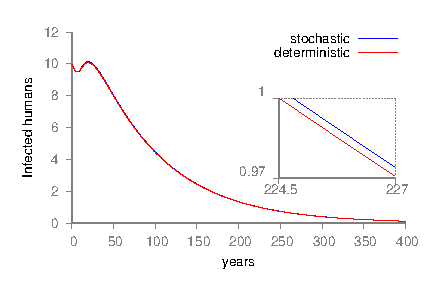
\includegraphics{%
			Sections/Section4/graphs/disease_free/disease_free_infected_humans.eps%
		}
	}
	\subfloat[][%
		Stochstic infected vector population.%
		]{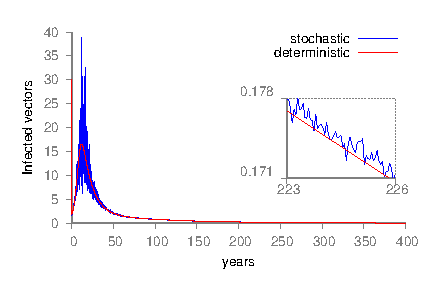
\includegraphics{%
		Sections/Section4/graphs/disease_free/disease_free_infected_vectors.eps%
	}%
	}
	\caption{
		A realization of the stochastic process solution under hypothesis of
		\Cref{theo:GSAS} for $t\in[0,400]~\si{years}$, see
		\Cref{tbl:initial_conditions,tbl:free_disease_parameters}
		for initial conditions and parameters values.
	}
	\label{fig:trajectories_free_desease}
\end{figure}
%%%%%%%%%%%%%%%%%%%%%%%%%%%%%%%%%%%%%%%%%%%%%%%%%%%%%%%%%%%%%%%%%%%%%%%%%%%%%%%%
%	Free disease moments
%
%
%%%%%%%%%%%%%%%%%%%%%%%%%%%%%%%%%%%%%%%%%%%%%%%%%%%%%%%%%%%%%%%%%%%%%%%%%%%%%%%%
\begin{figure}[p]
	\centering
	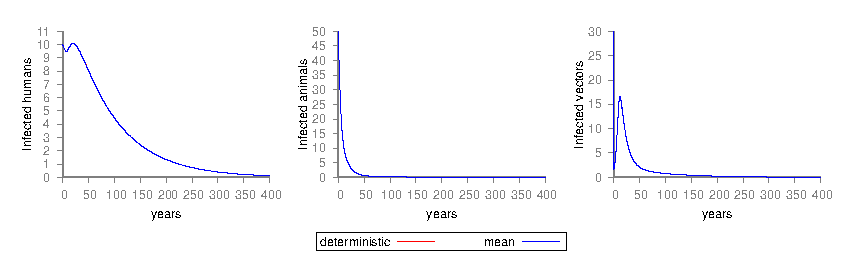
\includegraphics{%
		Sections/Section4/graphs/disease_free/disease_free_mean_population.eps%
		}%
	\caption{
		Numerical mean of \num{10000} solution trajectories
		under conditions of \Cref{theo:GSAS}.
	}
	\label{fig:mean_free_disease}
\end{figure}

\begin{figure}[p]
	\centering
	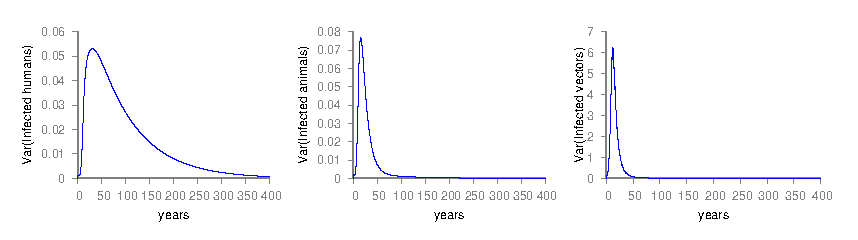
\includegraphics{%
		Sections/Section4/graphs/disease_free/disease_free_variance_population.eps%
	}
	\caption{
		Variance of \num{10000} solution trajectories under conditions of 
		\Cref{theo:GSAS}.
	}\label{fig:variance_free_disease}
\end{figure}
%%%%%%%%%%%%%%%%%%%%%%%%%%%%%%%%%%%%%%%%%%%%%%%%%%%%%%%%%%%%%%%%%%%%%%%%%%%%%%%%
%	Free disease exit time Histograms
%
%
%%%%%%%%%%%%%%%%%%%%%%%%%%%%%%%%%%%%%%%%%%%%%%%%%%%%%%%%%%%%%%%%%%%%%%%%%%%%%%%%
\begin{figure}[p]
	\centering
	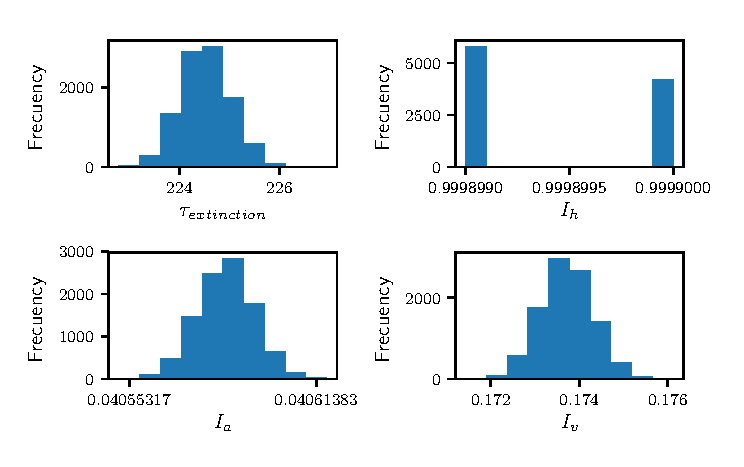
\includegraphics{%
		Sections/Section4/graphs/disease_free/stopping_time_histograms.eps%
	}
	\caption{
		Histograms of \num{10 000} sample paths under sufficient conditions for
		disease extinction see \Cref{theo:GSAS}
		and \Cref{tbl:free_disease_parameters}. As we  see at upper left, the 
		first time when all population are less than one $\tau_{extinction}$ 
		distributes its \num{10 000} occurrences around \num{220} and \num{230} 
		\si{years}.
	}\label{fig:extinction_stopping_time_histograms}
\end{figure}